\documentclass[a4paper, 12pt, finnish]{report} %dokumenttiluokka ja sille muutamia määrityksiä
\usepackage[utf8]{inputenc}
\usepackage{mathtools}
\usepackage{amsfonts}
%%\usepackage[toc,page]{appendix}
\usepackage{amsmath} %matematiikka kirjasto
\usepackage{graphicx} %kuvien liittämiseen kuten etusivun Aalto-logo
%\usepackage{pgfplots} %kuvaajien piirtämiseen, ota kommentointi pois mikäli haluat käyttää
\usepackage[finnish]{babel} %suomenkieli
\addto{\captionsfinnish}{\renewcommand{\bibname}{Lähteet}}
\usepackage{amsmath} %matematiikka kirjasto
\usepackage{graphicx} %kuvien liittämiseen kuten etusivun Aalto-logo
\usepackage{cite}
\usepackage[nottoc,numbib]{tocbibind}
\usepackage{titlesec}
\titleformat{\chapter}
{\Large\bfseries} % format
{}                % label
{0pt}             % sep
{\huge}           % before-code

\usepackage{hyperref}
\hypersetup{pdfpagemode=UseNone, pdfstartview=FitH, colorlinks=true,urlcolor=red,linkcolor=blue,citecolor=black,pdftitle={Kandityön suunnitelma},pdfauthor={Onni Lampi}}
%\usepackage{pgfplots} %kuvaajien piirtämiseen, ota kommentointi pois mikäli haluat käyttää

%\pagestyle{empty} %ei numeroita sivulle, mikäli niitä silti ilmestyy niin käytä komentoa \thispagestyle{empty} näillä sivuilla. Ei meinaa jostain syystä toimia report luokan kanssa
\setlength{\parindent}{0mm} %ei sisennystä uusiin kappaleisiin
\setlength{\emergencystretch}{15pt} %tekstin muokkaamiseen eli sallii välien venytyksen riveillä jotta näyttää paremmalta
\renewcommand{\bibname}{References}
\newcommand*{\findate}{\the\day.\the\month.\the\year} %uusi komento päivämäärän esittämiseen suomalaisittain
\newcommand*{\sijoitus}[2]{\mathop{\Big/}\limits_{\mspace{-19mu}#1}^{\mspace{19mu}#2}} % uusi komento jolla saadaan itgeraaliin suomalainen sijoitus viiva, käytetään \sijoitus{yläraja}{alaraja}, vaatii amsmath kirjaston
\renewcommand\thesection{\arabic{section}}
\usepackage{fancyhdr}
 
%\pagestyle{fancy}
%\fancyhf{}
%\rhead{Hekon logo}
%\lhead{Helsingin Kotkat ry - toimintakertomus 2015-2016}
\begin{document}

%\begin{center}
%
\includegraphics[width=50mm, scale=0.1]{heko.png}
%\end{center}
%\begin{center}
%	
\includegraphics[keepaspectratio=true,height=70mm]{heko.png}
%\end{center}
\chapter{Toimintakertomus 2016-2017}

\begin{figure}[htb]
	\begin{center}
	
\includegraphics[height=4cm]{heko.png}
	\end{center}
	%\caption{Kuvateksti, jossa on liitteen numerointi}
\end{figure}


\section{Yleistä lippukunnasta}
Helsingin Kotkat toteuttaa toiminnassaan Suomen Partiolaisten partio-ohjelmaa. Toiminta oli kuluneella kaudella aktiivista ja lippukunnan jäsenmäärä on vakaa.\\
\\Lippukunnassa toimi keväällä 2016 yksi tyttösudenpentulauma, kaksi poikasudenpentulaumaa, yksi tyttöseikkailijajoukkue, yksi poikatarpojajoukkue, yksi tyttötarpojaryhmä sekä yksi poikasamoajaryhmä.\\
\\Lisäksi lippukunnan johtajatehtävisä toimivat vaeltajat ja aikuiset ovat kokoontuneet toiminnansuunnittelun merkeissä.
\newpage
\section{Toiminta}
\subsection{Kokoukset}

\begin{figure}[htb]
	\begin{center}
	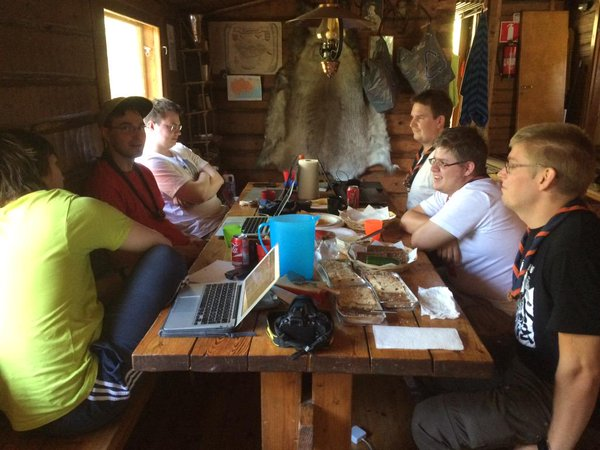
\includegraphics[height=6cm]{kokous.jpg}
	\end{center}
	\caption{Toiminnansuunnittelua lippukunnan kämpällä.}
\end{figure}


Ryhmät koontuivat omiin tapaamisiinsa viikoittain ja johtajat pitivät omia kokouksiaan tarpeen mukaan, esimerkiksi retkien suunnittelua varten. Kokouksista ja niiden määrästä lista alla:\\
\begin{center}
\begin{tabular}{ l l }
	Vuosikokous & 1 kpl\\
	Vaalikokous & 1 kpl\\
	Hallituksen kokous & 9 kpl\\
	Poikasamoajat & n kpl\\
	Tyttötarpojat & n kpl\\
	Tyttöseikkailijat & n kpl\\
	Poikaseikkailijat & n kpl\\
	Tyttösudenpennut & n kpl\\
	Poikasudenpennut & n kpl\\
			 & \\
	Yhteensä & x kpl\\
\end{tabular}
\end{center}
Lisäksi vuoden mittaan on pidettu lukuisia muita pienempiä ja epävirallisia kokouksia, joissa on esimerkiksi suunniteltu toimintaa, retkiä tai kämppien kunnostusta.
\section{Teoria, aineisto, menetelmä}
\section{Aikataulu kesälle 2017}
Alla aikataulua viikkotarkkuudella työn etenemisestä:
\begin{itemize}
	\item \textbf{Viikko 21:} Esitehtävän tekoa. Työkaluihin tutustumista (lähinnä LaTeX ja BibTeX)
	\item \textbf{Viikko 22:} Maanantaina ja tiistaina luentopäivät. Mahdollinen palaveri ohjaajan kanssa loppuviikosta.
	\item \textbf{Viikko 23:} Materiaalin keräämistä ja jäsentelyä. Teoriaosuuden ranka valmiiksi.
	\item \textbf{Viikko 24:} Teoriaosuuden vedos 1 valmiiksi, palautus perjantaina.
	\item \textbf{Viikko 25:} Palautteen pohjalta teoriaosuuden työstämistä parempaan kuntoon.
	\item \textbf{Viikko 26:} Lähdeluettelon viimeistely, kuvien tuottaminen. Case-studyn aloitus.
	\item \textbf{Viikko 27:} Sunnuntaina toisen vedoksen DL.
	\item \textbf{Viikko 28:} Pienryhmäkeskustelua toidesta vedoksesta. Tämän pohjalta parannuksia.
	\item \textbf{Viikko 29:} Maanantaina raportti pienryhmäkeskustelusta palautettu. Case-studyn tekninen toteutus tiedossa. Kolmas vedos palautetaan sunnuntaina.
	\item \textbf{Viikko 30:} Pienryhmäkeskustelua ja tämän raportointia. Case-studyn tekninen toteutus alkaa.
	\item \textbf{Viikko 31:} Neljäs vedos palautettava sunnuntaina. Tähän vedokseen jo alustavasti kuvia ja dataa case-studystä.
	\item \textbf{Viikko 32:} Teoriaosuuden viimeistely. Johtopäätöksiä case-studystä itse työhön.
	\item \textbf{Viikko 33:} Perjantaina kommentit ohjaahalta, näiden perusteella raivokasta työn parantelua.
	\item \textbf{Viikko 34:} Sunnuntaina seminaarikalvot valmiina. Näiden työstöä loppuviikosta.
	\item \textbf{Viikko 35:} Seminaariviikko.
	\item \textbf{Viikko 36:} Työn viimeistelyä.
	\item \textbf{Viikko 37:} Työn viimeistelyä, viimeinen DL palauttaa työ on tämän viikon sunnuntai.

















\end{itemize}
\clearpage
\nocite{*}

\end{document}
